\section{Vector Space Model}
Hệ thống khởi đầu bằng việc tiếp nhận tập hợp các tài liệu văn bản đầu vào. Đây có thể là các file văn bản độc lập hoặc một tập dữ liệu lớn như Cranfield. Các tài liệu này sẽ trải qua bước tiền xử lý nhằm chuẩn hóa nội dung, bao gồm các thao tác như chuyển về chữ thường, loại bỏ dấu câu và ký tự đặc biệt, tách từ, loại bỏ từ dừng và có thể áp dụng kỹ thuật stemming để rút gọn từ về gốc.

Sau khi tiền xử lý xong, hệ thống tiến hành xây dựng tập từ vựng (vocab) -- tức là danh sách tất cả các từ duy nhất xuất hiện trong tập tài liệu sau tiền xử lý. Mỗi từ trong từ vựng được ánh xạ với một mã số định danh duy nhất (term\_id). Từ đó, hệ thống xây dựng tập posting, trong đó mỗi từ được liên kết với danh sách các tài liệu mà nó xuất hiện, kèm theo tần suất hoặc trọng số (thường là TF-IDF). Tập hợp thông tin này được tổ chức thành một cấu trúc gọi là chỉ mục đảo (inverted index), cho phép tra cứu nhanh các tài liệu chứa một từ cụ thể.

Trong khi đó, truy vấn của người dùng -- dưới dạng một câu hỏi hoặc cụm từ -- cũng được đưa vào hệ thống. Truy vấn này sẽ được tiền xử lý theo quy trình tương tự như tài liệu, nhằm đảm bảo tính thống nhất trong biểu diễn. Sau tiền xử lý, truy vấn được chuyển thành vector trong cùng không gian với các tài liệu đã lập chỉ mục.

Khi đó, chỉ mục đảo được sử dụng như một cầu nối giữa truy vấn và các tài liệu. Dựa vào các từ khóa trong truy vấn, hệ thống truy xuất các tài liệu liên quan từ chỉ mục đảo, sau đó tiến hành tính toán mức độ tương đồng giữa vector truy vấn và vector tài liệu. Độ đo thường được sử dụng là độ tương đồng cosine, cho phép đánh giá mức độ gần nhau giữa các vector.

Cuối cùng, hệ thống xếp hạng các tài liệu theo độ tương đồng giảm dần và trả về danh sách các tài liệu phù hợp nhất với truy vấn. Đây là đầu ra của hệ thống -- tập hợp các văn bản được sắp xếp theo mức độ liên quan, giúp người dùng nhanh chóng tiếp cận thông tin cần thiết.

\begin{figure}[H]
    \centering
    \caption{Sơ đồ hệ thống của mô hình VSM}
    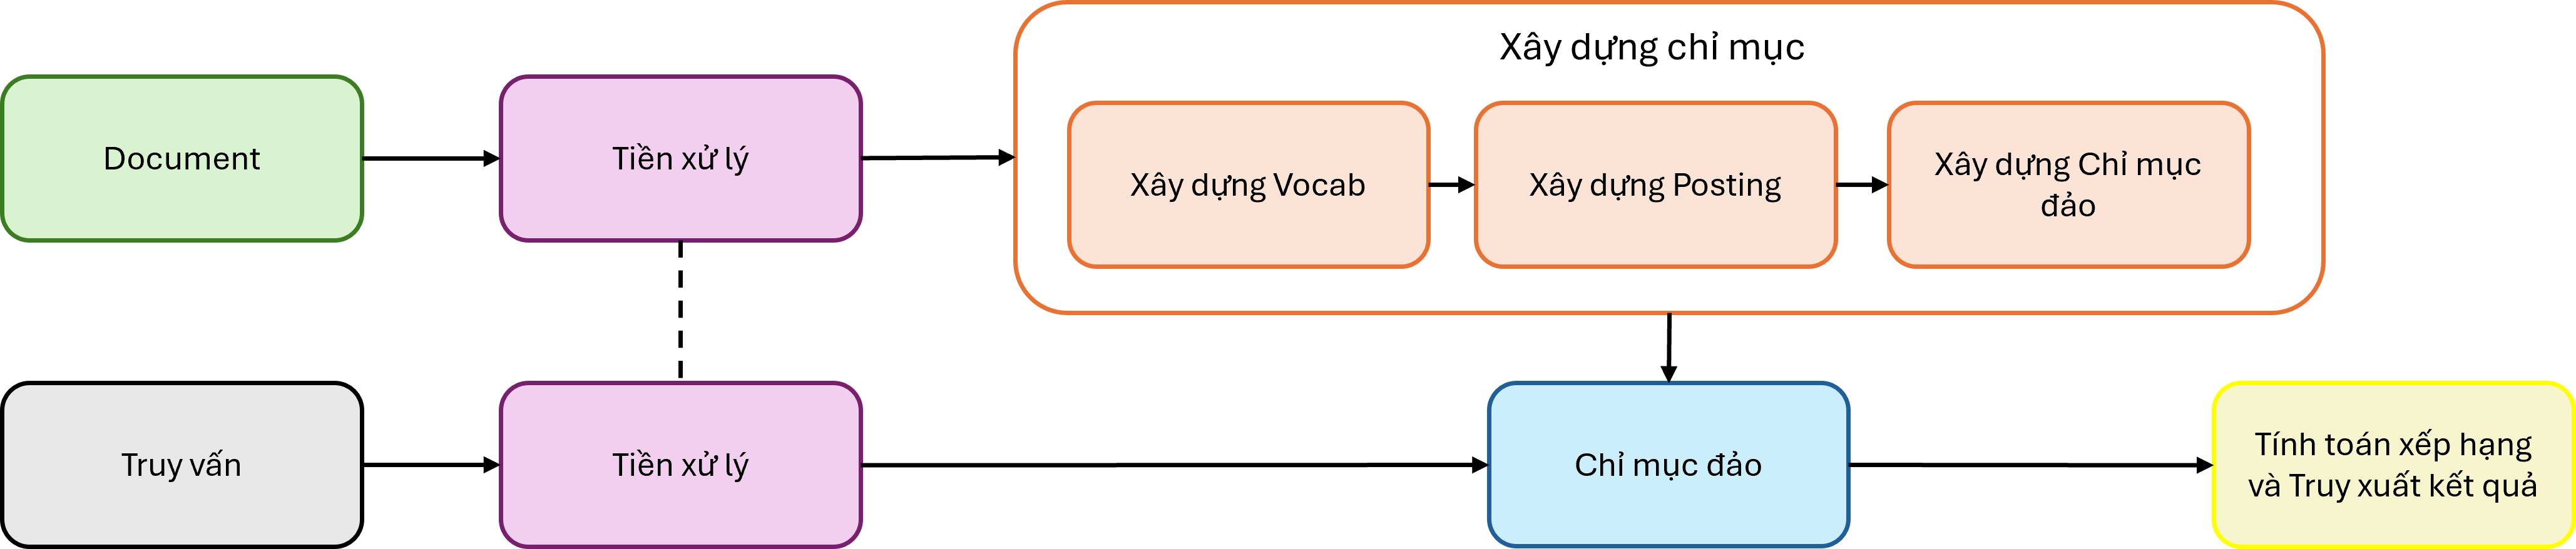
\includegraphics[width=\linewidth]{assets/vsm-flowchart.png}
\end{figure}

Để đánh giá mức độ hiệu quả của mô hình, nhóm đã thực nghiệm trên tập dữ liệu \textbf{Cranfield} --- một tập văn bản tiêu chuẩn thường được sử dụng trong các bài toán truy hồi thông tin. Trong quá trình tiền xử lý, nhóm đã thực hiện các bước làm sạch văn bản nhằm chuẩn hóa dữ liệu đầu vào và nâng cao chất lượng truy xuất. Cụ thể:

\begin{itemize}
    \item \textbf{Loại bỏ ký tự đặc biệt và dấu câu} nhằm loại bỏ nhiễu không cần thiết.
    \item \textbf{Loại bỏ stopwords} sử dụng tập từ dừng tiếng Anh chuẩn từ thư viện \texttt{nltk}, thông qua hàm \texttt{stopwords.words('english')}.
    \item \textbf{Stemming} được thực hiện bằng công cụ \texttt{SnowballStemmer} với ngôn ngữ tiếng Anh (\texttt{SnowballStemmer("english")}).
\end{itemize}

Không giống như các phương pháp stemming đơn giản hơn như \texttt{PorterStemmer}, công cụ \texttt{SnowballStemmer} (còn gọi là \textit{Porter2}) là một trình gốc hóa từ nâng cao được thiết kế để cân bằng giữa hiệu quả và độ chính xác. Ngoài chức năng chính là \textit{rút gọn từ về gốc}, \texttt{SnowballStemmer} còn có khả năng xử lý linh hoạt hơn đối với các quy tắc hậu tố phức tạp trong tiếng Anh, giúp quy các từ có chung gốc nghĩa như ``running'', ``ran'', ``runner'' về một biểu diễn thống nhất. Điều này góp phần làm giảm phân mảnh từ vựng và nâng cao độ chính xác của truy vấn.

Sau khi hoàn tất bước tiền xử lý và xây dựng chỉ mục theo mô hình Vector Space Model (VSM), nhóm đã thu được các thống kê tổng quát như sau:

\begin{itemize}
    \item \textbf{Tổng số văn bản (documents)}: 1400
    \item \textbf{Kích thước từ vựng (vocabulary size)}: 4672
    \item \textbf{Tổng số postings (số lượng cặp term--document)}: 86,680
    \item \textbf{Số postings trung bình trên mỗi từ}: 18.55
\end{itemize}

Những thống kê này cho thấy hệ thống chỉ mục đã được xây dựng hiệu quả, với một từ trung bình xuất hiện trong khoảng 18 tài liệu, phản ánh mức độ phổ biến của các từ trong tập dữ liệu và ảnh hưởng trực tiếp đến khả năng truy hồi tài liệu của hệ thống.

Sau khi xây dựng chỉ mục và triển khai mô hình Vector Space Model (VSM), nhóm đã thực nghiệm truy vấn trên tập dữ liệu Cranfield nhằm đánh giá hiệu quả của hệ thống truy xuất. Các chỉ số đánh giá được sử dụng bao gồm Precision@10, Recall@10, Mean Average Precision (MAP) và đường cong Precision-Recall theo chuẩn TREC.

\begin{itemize}
    \item \textbf{Mean Precision@10}: 0.2271
    \item \textbf{Mean Recall@10}: 0.3922
    \item \textbf{Mean Average Precision (MAP)}: 0.2685
\end{itemize}

Những chỉ số này cho thấy mô hình VSM có khả năng truy xuất ở mức độ tương đối, với độ chính xác trung bình ở top 10 kết quả là khoảng 22.71\% và độ bao phủ (recall) ở mức 39.22\%. Giá trị MAP phản ánh hiệu quả tổng thể của mô hình trên toàn bộ tập truy vấn.
